\section[Puissance des forces de frottement]{Puissance instantanée des forces de frottement de glissement}

    \subsection{Puissance totale instantanée des forces liées aux actions de contact entre deux solides}

        On considère le système présenté à la Figure~\ref{fig:systeme_force_frottement_glissement}.

        \begin{figure}
            \centering
            \tikzsetnextfilename{systeme_force_frottement_glissement}
            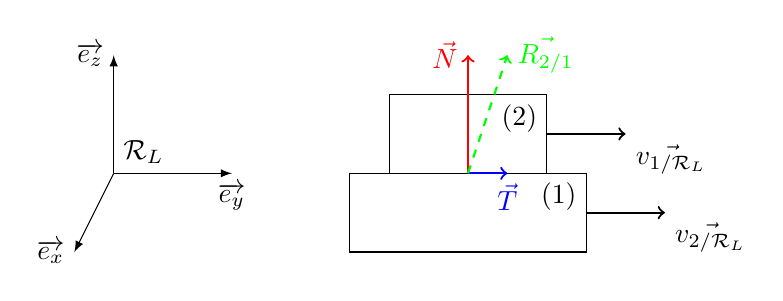
\begin{tikzpicture}[scale=1]  

                \draw (0,0) rectangle++(3,1) node [below left] {$(1)$};
                \draw (0.5,1) rectangle++(2,1) node [below left] {$(2)$};
                \draw [->, blue, thick] (1.5,1) --++ (0.5,0) node [below] {$\vec{T}$};
                \draw [->, red, thick] (1.5,1) --++ (0,1.5) node [left] {$\vec{N}$};
                \draw [->, green, thick, dashed] (1.5,1) --++ (0.5,1.5) node [right] {$\vec{R_{2/1}}$};

                \draw [->, thick] (3,0.5) --++ (1,0) node [below right] {$\vec{v_{2/\mathcal{R}_L}}$};
                \draw [->, thick] (2.5,1.5) --++ (1,0) node [below right] {$\vec{v_{1/\mathcal{R}_L}}$};

                \draw [->,-latex] (-3,1) --++ (-0.5,-1) node [left] {$\overrightarrow{e_x}$}	;   
                \draw [->,-latex] (-3,1) --++ (1.5,0) node [below] {$\overrightarrow{e_y}$}	;
                \draw [->,-latex] (-3,1) --++ (0,1.5) node [left] {$\overrightarrow{e_z}$}	; 
                \node at (-3,1) [above right] {$\mathcal{R}_L$};      

            \end{tikzpicture}
            \caption{Système modèle pour l'étude de la puissance des forces de frottement de glissement.}
            \label{fig:systeme_force_frottement_glissement}
        \end{figure}

        On a $\left(P_{2\to1}\right)_{/\mathcal{R}_L}=\vec{R_{2/1}}\cdot\vec{v_{1/\mathcal{R}_L}}$ et $\left(P_{1\to2}\right)_{/\mathcal{R}_L}=\vec{-R_{2/1}}\cdot\vec{v_{2/\mathcal{R}_L}}$. Ainsi, la puissance totale est
        \begin{equation*}
            P_{\text{tot}}=\vec{R_{2/1}}\cdot\left(\vec{v}_{1}-\vec{v}_2\right)=\vec{R_{2/1}}\cdot\vec{v_g}_{(1/2)}=\vec{T}\cdot\vec{v_g}_{(1/2)}\leqslant 0.
        \end{equation*}

        \paragraph{Condition pour aoivr $P_{\text{tot}}=0$.}

            On a 
            \begin{itemize}
                \item soit $\vec{T}=\vec{0}$ : il y a glissement sans frottement $(f_d=0)$ (exemple : ski, patinage);
                \item soit $\vec{v}_g=\vec{0}$ : il y a roulement sans glissement (exemple : voiture qui démarre sans les roues qui patinent, freinage sans blocage).
            \end{itemize} 

    \subsection{Exemple d'un pavé mis en mouvement par un tapis roulant : bilan énergétique}

        On considère une boîte $b$ mise sur un tapis roulant $t$ dans un supermarché, comme décrit à la Figure~\ref{fig:pave_tapis_roulant_bilan_energetique}. On fait l'hypothèse que $u>v$, ainsi on a $\vec{v}_g(b/t)=(v-u)\vec{u_x}$, d'où $\vec{T}=T\vec{u_x}$ avec $T>0$.

        \begin{figure}
            \centering
            \tikzsetnextfilename{pave_tapis_roulant_bilan_energetique}
            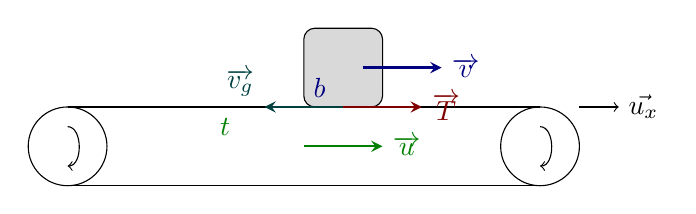
\begin{tikzpicture}[scale=1]  
                % \helpgrid{3}{3}
                \draw (-3,0) -- (3,0) ;  
                \draw (-3,-1) -- (3,-1) ;  
                \draw [->] (3.5,0) -- (4,0) node [right] {$\vec{u_x}$};  
                \coordinate (M) at (0,0);
                \draw[rounded corners=4pt,fill=gray!30] (0,0) rectangle++ (1,1) node [midway, shift=({0,0.05})] {$\centerdot$}; 
                \draw [->,-stealth,thick,blue!50!black] (M)++(0.75,0.5)--++(1,0) node [right] {$\overrightarrow{v}$};
                \draw [->,-stealth,thick,green!50!black] (M)++(0,-0.5) --++(1.,0) node [right] {$\overrightarrow{u}$};
                \draw [->,-stealth,thick,red!50!black] (M)++(0.5,0) --++(1.,0) node [right] {$\overrightarrow{T}$};
                \draw [->,-stealth,thick,teal!50!black] (M)++(0.5,0) --++(-1.,0) node [above left] {$\overrightarrow{v_g}$};
                \node[text=blue!50!black] at (M) [above right] {$b$};
                \node[text=green!50!black] at (-1,-0.25) {$t$};
                \draw [color=black,smooth] (-3,-0.5) circle (0.5);
                \draw [color=black,smooth] (3,-0.5) circle (0.5);
                \draw [->] (-3,-0.25) to [bend left=90] (-3,-0.75);
                \draw [->] (3,-0.25) to [bend left=90] (3,-0.75);

            \end{tikzpicture}
            \caption{Pavé mis en mouvement par un tapis roulant.}    
            \label{fig:pave_tapis_roulant_bilan_energetique}
        \end{figure}

        Les valeurs des différentes puissances des forces de frottements de glissement selon le référentiel choisi sont données dans la Table~\ref{tab:puissance_tapis_roulant_supermarche}.

        \begin{table}
            \centering
            \begin{tabular}{c|c|c|c}
                \toprule
                & $\mathcal{R}_{\text{supermarché}}$ & $\mathcal{R}_{\text{tapis}}$ & $\mathcal{R}_{\text{boîte}}$  \\ \midrule
                $P_{t\to b}$ & $T\times v>0$ & $T\times(v-u)<0$ & $T\times0=0$\\ \midrule
                $P_{b\to t}$ & $(-T)\times u<0$ & $(-T)\times 0 = 0$& $(-T)\times(u-v)>0$\\ \midrule
                $P_{\text{tot}}$ & $T\times(v-u)=T\times v_g<0$ & $T\times(v-u)<0$ & $T\times(v-u)<0$\\ \bottomrule
            \end{tabular}    
            \caption{Puissance des forces de frottements de glissement selon certains référentiels.}
            \label{tab:puissance_tapis_roulant_supermarche}
        \end{table}

        Ainsi, même si elle sont motrices, les forces de frottement sont toujours globalement dissipatives : $P_{\text{tot}}<0$. $P_{\text{tot}}$ est indépendant du référentiel d'étude.
        On peut généraliser le résultat : les puissances intérieures $P_{\text{int}}$ sont indépendantes du référentiel (en prenant la réunion des deux systèmes boîte/tapis).
